\chapter{Gebrochene Symmetrie, Goldstone-Bosonen und Eichinvarianz}

Wir wollen verstehen, wie ein photonartiges Teilchen eine Masse erhalten kann. Das ist das Ziel, aber kein sinnvoller Ausgangspunkt. Ein direkter Massenterm für ein Eichfeld scheint gerade jene Eichinvarianz zu zerstören, die die Konsistenz der Theorie gewährleistet. Bevor wir den Ausweg erkennen können, müssen wir zwei Ideen in ihrer konkreten Form verstehen:
\begin{enumerate}
  \item spontane Symmetriebrechung, insbesondere bei einer kontinuierlichen Symmetrie;
  \item Eichinvarianz, bei der die Symmetrieoperation von einem Raumzeitpunkt zum anderen variieren darf.
\end{enumerate}
Keine der beiden Ideen lässt sich durch einen bloßen Merksatz ersetzen. Wir entwickeln die erste anhand eines Magneten, übertragen sie auf die Theorie skalarer Felder und entdecken den masselosen Goldstone-Modus. Dann machen wir dieselbe \(U(1)\)-Symmetrie lokal, was uns zwingt, ein Vektorpotential und eine kovariante Ableitung einzuführen. Erst am Ende stellen wir die beiden Gedankengänge nebeneinander. Ihre tatsächliche Verbindung---das Higgs-Phänomen---ist Thema der nächsten Vorlesung.

\section{Ein symmetrisches Gesetz mit einem asymmetrischen Grundzustand}

\subsection{Der Zweizustandsmagnet}

Betrachten wir ein Gitter aus kleinen Magneten. Jeder Spin kann nach oben oder unten zeigen, und benachbarte Spins haben eine geringere Energie, wenn sie in dieselbe Richtung zeigen. Auf einem dreidimensionalen kubischen Gitter hat ein Spin sechs nächste Nachbarn, doch die genaue Koordinationszahl ist unwichtig. Entscheidend ist die Regel
\begin{equation}
  E_{\parallel}<E_{\rm antiparallel}.
\end{equation}
Die mikroskopische Regel bleibt unverändert, wenn alle Spins umgekehrt werden:
\begin{equation}
  \uparrow\longleftrightarrow\downarrow.
\end{equation}
Dennoch sind die Konfigurationen niedrigster Energie nicht jeweils für sich symmetrisch. Sie lauten
\begin{equation}
  \{\uparrow\uparrow\uparrow\cdots\},
  \qquad
  \{\downarrow\downarrow\downarrow\cdots\}.
\end{equation}
Die Gleichungen erlauben beide, doch eine kalte makroskopische Probe muss sich für eine davon entscheiden.

Diese Wahl ist außerordentlich empfindlich. Wir fixieren einen sehr weit entfernten Spin so, dass er nach oben zeigt. Seine Nachbarn richten sich bevorzugt nach ihm aus, deren Nachbarn wiederum nach ihnen, und die Information breitet sich durch die Probe aus. Eine Störung, die im Vergleich zum Gesamtsystem beliebig klein ist, kann die Orientierung des gesamten Grundzustands festlegen. Das ist die Instabilität, die mit \emph{spontan}er Symmetriebrechung gemeint ist.

\begin{classroomqa}
\audiencequestion{Kann ein neutrales Teilchen sich in einem Magnetfeld ausrichten?
\lecturetimestamp{00:05:14}}
\lecturerresponse{Ja. Elektrische Neutralität bedeutet nicht, dass kein magnetisches Moment vorhanden ist. Das Neutron ist neutral, besitzt aber aufgrund seiner inneren geladenen Bestandteile ein magnetisches Moment. Ein Magnetfeld kann daher zwischen seinen Spinorientierungen unterscheiden.}
\end{classroomqa}

\begin{classroomqa}
\audiencequestion{Wenn das System seine Orientierung ändert, geschieht das dann überall gleichzeitig? Können mehrere Umorientierungswellen nebeneinander bestehen?
\lecturetimestamp{00:05:41--00:06:38}}
\lecturerresponse{Die Änderung breitet sich aus. Ein Bereich kippt seine Nachbarbereiche, ähnlich wie bei einem dreidimensionalen Dominofeld, und die Störung wandert als Welle weiter. Verschiedene Bereiche können unabhängig voneinander mit ihrer Wahl beginnen, sodass mehrere Fronten und mehrere Domänen vorhanden sein können, bevor sich eine Orientierung durchsetzt. Auf genau diese Wellen kommen wir zurück, wenn die Symmetrie kontinuierlich wird.}
\end{classroomqa}

\subsection{Explizite Brechung ist eine andere Theorie}

Bringen wir die Probe nun in ein externes, nach oben gerichtetes Magnetfeld. Ein isolierter Spin hat bereits eine niedrigere Energie, wenn er nach oben zeigt. Die Transformation \(\uparrow\leftrightarrow\downarrow\) lässt die Energie nicht länger unverändert: Die Bevorzugung ist in das Gesetz selbst eingebaut. Das ist \emph{explizite}Symmetriebrechung.

Der Unterschied lässt sich prüfen, ohne zu wissen, wie die Probe präpariert wurde. Wir nehmen eine sehr große Probe, halten ihren linken Rand nach oben und ihren rechten Rand nach unten. Bevorzugt ein magnetisches Bulk-Feld explizit die Ausrichtung nach oben, dringt die Randbedingung am rechten Ende nur ein kurzes Stück weit ein. Eine makroskopische Region mit Ausrichtung nach unten würde eine Energie kosten, die proportional zu ihrem Volumen ist; das Bulk kann daher nicht in zwei gleichwertige Phasen unterteilt bleiben.

Ohne äußere Bevorzugung haben die Ausrichtungen nach oben und nach unten dieselbe Bulk-Energie. Der Zustand niedrigster Energie unter den Randbedingungen enthält dann eine Domäne mit Ausrichtung nach oben, eine mit Ausrichtung nach unten und eine endliche Übergangsschicht dazwischen. Die Grenzfläche muss nicht genau in der geometrischen Mitte liegen, doch es gibt keinen Volumendruck, der eine Phase dazu zwingt, die andere zu beseitigen. Diese Grenzfläche ist eine \emph{Domänenwand}, die charakteristische Defektstruktur dieser gebrochenen diskreten Symmetrie.

\begin{figure}[htbp]
\centering
\begin{adjustbox}{max width=\linewidth}
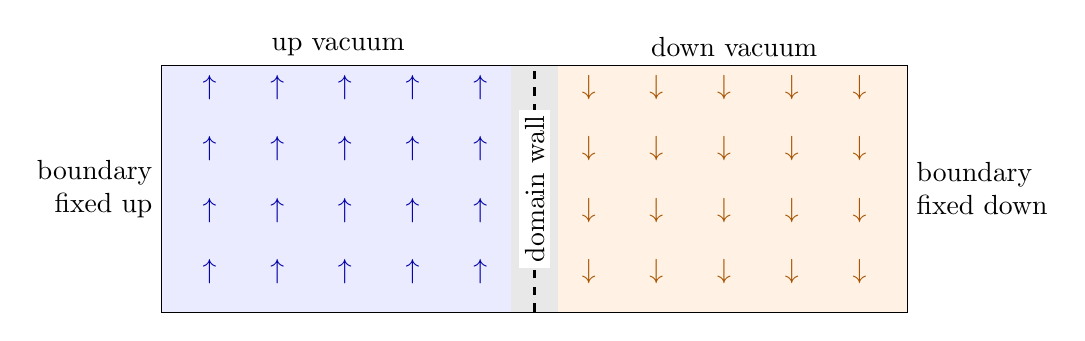
\begin{tikzpicture}[x=0.86cm,y=0.78cm]
  \draw[thick] (0,0) rectangle (11,4);
  \fill[blue!8] (0,0) rectangle (5.15,4);
  \fill[orange!10] (5.85,0) rectangle (11,4);
  \fill[gray!18] (5.15,0) rectangle (5.85,4);
  \foreach \x in {0.7,1.7,2.7,3.7,4.7}
    \foreach \y in {0.65,1.65,2.65,3.65}
      \node[blue!65!black] at (\x,\y) {$\uparrow$};
  \foreach \x in {6.3,7.3,8.3,9.3,10.3}
    \foreach \y in {0.65,1.65,2.65,3.65}
      \node[orange!65!black] at (\x,\y) {$\downarrow$};
  \draw[dashed,thick] (5.5,0) -- (5.5,4);
  \node[above] at (2.6,4) {up vacuum};
  \node[above] at (8.45,4) {down vacuum};
  \node[rotate=90,fill=white,inner sep=2pt] at (5.5,2) {domain wall};
  \node[left,align=right] at (0,2) {boundary\\fixed up};
  \node[right,align=left] at (11,2) {boundary\\fixed down};
\end{tikzpicture}
\end{adjustbox}
\caption{Der Randbedingungstest für die spontane Brechung einer diskreten Symmetrie. Beide Bulk-Orientierungen haben dieselbe Energie, daher kann eine Wand makroskopische Domänen voneinander trennen.}
\end{figure}

\begin{classroomqa}
\audiencequestion{Erfordert das Argument, dass Wechselwirkungen nur zwischen nächsten Nachbarn auftreten?
\lecturetimestamp{00:18:18}}
\lecturerresponse{Nein. Eine Wechselwirkung mit zweitnächsten Nachbarn, die ebenfalls parallele Ausrichtung begünstigt, ändert zwar Details, nicht aber die Schlussfolgerung. Interessanter wird das Verhalten, wenn Wechselwirkungen verschiedener Reichweite miteinander konkurrieren---zum Beispiel, wenn nächste Nachbarn parallele Ausrichtung und übernächste Nachbarn antiparallele Ausrichtung bevorzugen. Das führt zu Frustration und komplizierteren geordneten Phasen, ändert aber nichts an der grundlegenden Unterscheidung, um die es hier geht.}
\end{classroomqa}

\begin{classroomqa}
\audiencequestion{Bezieht sich \emph{spontan}auf den großen Gradienten innerhalb der Wand?
\lecturetimestamp{00:19:05}}
\lecturerresponse{Nein. Gemeint ist, dass die zugrunde liegende Energie keine Bevorzugung von oben--gegenüber unten aufweist, der gewählte Grundzustand aber schon. Die dramatische Reaktion auf eine beliebig kleine Störung macht die Instabilität sichtbar. Der Gradient sagt lediglich aus, wie viel Energie die Grenzfläche kostet.}
\end{classroomqa}

\begin{classroomqa}
\audiencequestion{Befand sich das Material bereits in einem der beiden Zustände, oder war sein Zustand anfangs unbekannt?
\lecturetimestamp{00:19:40}}
\lecturerresponse{Das hängt von seiner Vorgeschichte ab. Bei hoher Temperatur kann die thermische Bewegung die Spins nach oben und unten mischen, sodass die mittlere Magnetisierung nahezu null ist. Kühlt das Material ab, nehmen verschiedene Bereiche unterschiedliche Orientierungen an, Domänenwände entstehen und die Domänen wachsen. Zufall und winzige Störungen aus der Umgebung entscheiden darüber, welches Vakuum schließlich den größten Teil der Probe einnimmt.}
\end{classroomqa}

\section{Dasselbe Argument in der Theorie skalarer Felder}

Ersetzen wir die Spins durch ein reelles Skalarfeld \(\phi(\bm{x},t)\). Bei festgelegten Metrik- und Normierungskonventionen schreiben wir
\begin{equation}
\begin{aligned}
  \mathcal L
  &=\frac12\,\partial_\mu\phi\,\partial^\mu\phi-V(\phi),
  \\
  \mathcal E
  &=\frac12\dot\phi^{\,2}+\frac12(\nabla\phi)^2+V(\phi).
\end{aligned}
  \label{eq:l07-real-scalar}
\end{equation}
Die relativistische Kurzschreibweise in \(\mathcal L\) enthält den positiven Zeitableitungsterm und den negativen räumlichen Gradiententerm; in der Hamiltonschen Energiedichte sind beide Beiträge positiv.

Wir wählen ein gerades Potential mit zwei entarteten Minima,
\begin{equation}
  V(\phi)=\frac{\lambda}{4}\left(\phi^2-f^2\right)^2,
  \qquad \lambda>0.
  \label{eq:l07-double-well}
\end{equation}
Die Lagrange-Dichte ist invariant unter \(\phi\mapsto-\phi\), während jedes der homogenen Vakua
\begin{equation}
  \phi(\bm{x})=+f,
  \qquad\hbox{or}\qquad
  \phi(\bm{x})=-f
\end{equation}
eine Seite auswählt. Ein Potential mit einem einzigen Minimum bei \(\phi=0\) hat dagegen ein symmetrisches Vakuum und ist nicht spontan gebrochen.

Wir fixieren \(\phi=+f\)auf der einen Seite einer Probe und \(\phi=-f\)auf der anderen. Das Feld kann nicht sprunghaft wechseln, ohne dass dies Energie kostet, denn
\begin{equation}
  E_{\rm wall}
  =\int dx\left[
      \frac12\left(\frac{d\phi}{dx}\right)^2+V(\phi)-V(f)
    \right].
  \label{eq:l07-wall-energy}
\end{equation}
Ein abrupter Sprung macht \(d\phi/dx\)sehr groß. Die Wand niedrigster Energie verteilt die Änderung daher über eine endliche Breite und gleicht dabei die Gradientenenergie gegen die potenzielle Energie ab, die beim Übergang zwischen den Minima anfällt. Die bekannte Kink-Lösung für das Potential in Gl.~\eqref{eq:l07-double-well}lautet
\begin{equation}
  \phi_{\rm wall}(x)
  =f\tanh\!\left[f\sqrt{\frac{\lambda}{2}}\,(x-x_0)\right],
  \label{eq:l07-kink}
\end{equation}
Sie veranschaulicht konkret den glatten Übergang, der an der Tafel beschrieben wurde.
\editorialnote{Die Vorlesung argumentiert anhand der Form des Potentials und des Gradiententerms, löst aber nicht die Feldgleichung. Gleichung \eqref{eq:l07-kink} ist als Standardlösung des angegebenen Modells aufgenommen und macht die qualitative Beschreibung der Wand konkret, ohne das Argument zu verändern.}

Verkippen wir das Doppelmuldenpotential leicht, wird eines der Minima tiefer. Die Lagrange-Dichte ist dann selbst asymmetrisch. Eine Wand kann vorübergehend weiterhin auftreten, doch das höherenergetische, falsche Vakuum übt einen Druck auf sie aus; die Wand bewegt sich und die bevorzugte Phase breitet sich aus. Das ist das feldtheoretische Gegenstück zur expliziten Brechung durch ein äußeres Magnetfeld.

Bislang war die Symmetrie diskret. Die Teilchenphysik wird von kontinuierlichen Gruppen wie \(U(1)\), \(SU(2)\)und \(SU(3)\)beherrscht. Eine kontinuierliche Symmetrie verändert die Geschichte der Defekte und führt eine neue Art von Teilchen ein.

\section{Ein komplexes Feld und globale \texorpdfstring{\(U(1)\)}{U(1)}}

\subsection{Drehungen in einer inneren Ebene}

Sei
\begin{equation}
  \phi=\phi_R+i\phi_I,
  \qquad
  \phi^*=\phi_R-i\phi_I,
  \qquad
  \phi^*\phi=\phi_R^2+\phi_I^2.
  \label{eq:l07-components}
\end{equation}
Die Achsen \(\phi_R\)und \(\phi_I\)bilden einen inneren Feldraum, keine zwei Richtungen im gewöhnlichen Raum. Ein komplexes Skalarfeld ist einfach eine Zusammenfassung zweier reeller Skalarfelder, die Drehungen in dieser inneren Ebene direkt erkennen lässt.

\begin{figure}[htbp]
\centering
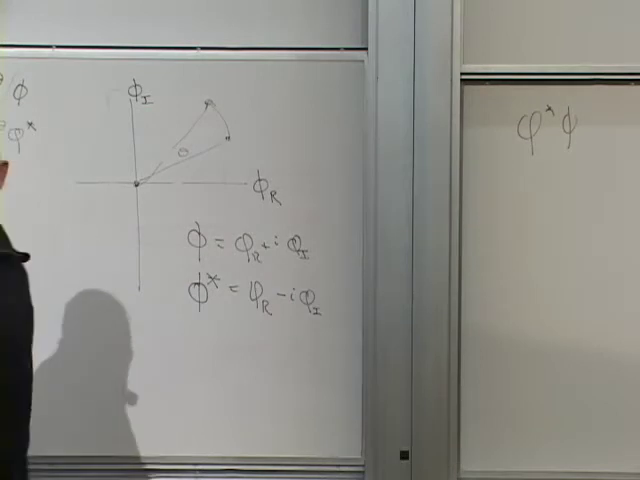
\includegraphics[width=0.80\textwidth]{lecture_07_figure_02.png}
\caption{Das komplexe Feld in der inneren \((\phi_R,\phi_I)\)-Ebene. An der Tafel werden die Zerlegung von \(\phi\)und \(\phi^*\)sowie der invariante Radius \(\phi^*\phi\)festgehalten.}
\lectureframe{00:33:33}
\end{figure}

Wir verwenden die Lagrange-Dichte
\begin{equation}
  \mathcal L
  =\partial_\mu\phi^*\,\partial^\mu\phi
   -V(\phi^*\phi).
  \label{eq:l07-complex-lagrangian}
\end{equation}
Bei einem komplexen Feld entfällt der übliche Faktor \(1/2\), denn dieses eine Produkt enthält bereits die kinetischen Terme beider reeller Komponenten. Die Transformation
\begin{equation}
  \phi'(x)=e^{i\theta}\phi(x),
  \qquad
  \phi^{*\prime}(x)=e^{-i\theta}\phi^*(x)
  \label{eq:l07-global-u1}
\end{equation}
dreht jeden Feldwert um denselben Winkel. Hier ist \(\theta\)räumlich und zeitlich konstant. Der Strich kennzeichnet das transformierte Feld; er steht nicht für eine Ableitung.

Da \(\theta\)konstant ist, gilt
\begin{equation}
  \partial_\mu\phi'=e^{i\theta}\partial_\mu\phi,
  \qquad
  \partial_\mu\phi^{*\prime}
  =e^{-i\theta}\partial_\mu\phi^*.
\end{equation}
Die Phasen heben sich im kinetischen Term auf, und
\(\phi^{*\prime}\phi'=\phi^*\phi\). Jedes Potential, das nur von \(\phi^*\phi\)abhängt, besitzt daher dieselbe Symmetrie. Ein Term, der allein von \(\phi_R\)abhängt, würde eine Richtung in der inneren Ebene auszeichnen und die Symmetrie explizit brechen.

\subsection{Ein punktförmiges Minimum und ein Kreis von Minima}

Es gibt zwei qualitativ verschiedene symmetrische Potentiale. Das erste hat sein einziges Minimum im Ursprung, zum Beispiel
\begin{equation}
  V_{\rm unbroken}=m^2\phi^*\phi,
  \qquad m^2>0.
\end{equation}
Sein Graph ist ein rotationssymmetrisches Paraboloid. Das Vakuum \(\phi=0\)bleibt unter jeder Drehung unverändert, die Symmetrie ist also ungebrochen.

Wählen wir nun
\begin{equation}
  V_{\rm broken}
  =-a\,\phi^*\phi+b(\phi^*\phi)^2,
  \qquad a,b>0.
  \label{eq:l07-mexican-hat}
\end{equation}
Der negative quadratische Term treibt das Feld vom Ursprung weg, während der positive quartische Term verhindert, dass es ins Unendliche läuft. Mit \(r^2=\phi^*\phi\)ergibt die Minimierung
\begin{equation}
  \frac{dV}{d(r^2)}=-a+2br^2=0,
  \qquad
  r^2=f^2=\frac{a}{2b}.
  \label{eq:l07-vacuum-radius}
\end{equation}
Die Minima bilden daher einen Kreis. Das Potential ist vollkommen rotationssymmetrisch, und doch muss ein homogener Grundzustand einen Punkt auf diesem Kreis auswählen.

\begin{figure}[htbp]
\centering
\includegraphics[width=0.72\textwidth]{lecture_07_figure_06.png}
\caption{Das Potential mit gebrochener Symmetrie als Rotationsfläche dargestellt. Der Ursprung ist instabil, und die entarteten Minima bilden die kreisförmige Rinne.}
\lectureframe{00:37:25}
\end{figure}

Man stelle sich das Feld an jedem Punkt des gewöhnlichen Raums als kleinen Pfeil in dieser inneren Ebene vor. Das Potential verlangt, dass jeder Pfeil die Länge \(f\)hat. Die Gradientenenergie verlangt, dass benachbarte Pfeile nahezu in dieselbe Richtung zeigen. Der Grundzustand hat folglich überall denselben Winkel, obwohl das Gesetz keinen Winkel bevorzugt. Das ist spontane Brechung einer kontinuierlichen Symmetrie.

\section{Von der Domänenwand zur glatten Verdrehung}

Wiederholen wir das Randbedingungsexperiment. Am linken Rand fixieren wir das Feld bei einem Vakuumpunkt \(A\); am rechten Rand fixieren wir es bei einem anderen Vakuumpunkt \(B\). Ein lokalisierter Sprung würde den Gradienten groß machen. Anders als im diskreten Fall kann das Feld jedoch am tiefsten Punkt des Potentials bleiben und sich dabei kontinuierlich um den Kreis bewegen.

Bei niedriger Energie schreiben wir das Feld als \(\phi=f e^{i\alpha(x)}\). In einer Raumdimension lautet die relevante Energie
\begin{equation}
  E[\alpha]
  =f^2\int_0^L dx\,\left(\frac{d\alpha}{dx}\right)^2.
  \label{eq:l07-angle-functional}
\end{equation}
Bei festgehaltenen Endwinkeln ergibt die Variation
\begin{equation}
  \frac{d^2\alpha}{dx^2}=0,
  \qquad
  \alpha(x)=\alpha_A+
    \frac{\alpha_B-\alpha_A}{L}\,x.
  \label{eq:l07-linear-twist}
\end{equation}
Die bevorzugte Konfiguration verteilt die Verdrehung gleichmäßig über die Probe. Ihre Energie skaliert wie
\begin{equation}
  E_{\rm twist}
  =f^2\frac{(\alpha_B-\alpha_A)^2}{L},
  \label{eq:l07-twist-energy}
\end{equation}
und lässt sich daher durch Vergrößern von \(L\)beliebig klein machen.

\begin{figure}[htbp]
\centering
\begin{adjustbox}{max width=\linewidth}
\begin{tikzpicture}[x=0.95cm,y=0.95cm]
  \begin{scope}
    \draw[->] (0,0) -- (6.2,0) node[right] {$x$};
    \draw[->] (0,0) -- (0,3.5) node[above] {$\alpha(x)$};
    \draw[very thick,blue!70!black] (0.45,0.65) -- (5.7,2.85);
    \fill (0.45,0.65) circle (1.8pt) node[left] {$\alpha_A$};
    \fill (5.7,2.85) circle (1.8pt) node[right] {$\alpha_B$};
    \node at (3.1,-0.65) {physical space};
  \end{scope}
  \begin{scope}[xshift=9.2cm,yshift=1.65cm]
    \draw[thick] (0,0) circle (1.8);
    \fill (1.55,-0.92) circle (1.8pt) node[below right] {$A$};
    \fill (-0.45,1.74) circle (1.8pt) node[above] {$B$};
    \draw[very thick,blue!70!black,-{Latex[length=2.5mm]}]
      (1.55,-0.92) arc[start angle=-31,end angle=104,radius=1.8];
    \node at (0,-2.35) {vacuum circle};
  \end{scope}
\end{tikzpicture}
\end{adjustbox}
\caption{Dieselbe Konfiguration niedriger Energie in zwei Darstellungen. Der Winkel variiert linear über den physikalischen Raum, während das Feld dem kurzen Kreisbogen des Vakuumkreises im inneren Raum folgt.}
\end{figure}

\begin{classroomqa}
\audiencequestion{Es gibt zwei Wege um den Kreis. Welchen Weg nimmt das Feld, und kann es auf dem längeren Weg gefangen bleiben?
\lecturetimestamp{00:41:54}}
\lecturerresponse{Für allgemeine Endpunkte hat der kürzere Weg entlang des Winkels den kleineren Gradienten und damit die niedrigere Energie. Bei diametral gegenüberliegenden Endpunkten sind die beiden einfachsten Wege entartet. Eine Konfiguration, die dadurch vorbereitet wurde, dass ein Endpunkt langsam bewegt wurde, kann eine zusätzliche Windung beibehalten und hinter einer Energiebarriere gefangen bleiben; für ein vorgegebenes Paar gewöhnlicher Endpunkte ist jedoch der unverdrillte kürzeste Weg der Grundzustand.}
\end{classroomqa}

\begin{classroomqa}
\audiencequestion{Könnte der Weg den Grund der Rinne verlassen und quer durch ihr Inneres verlaufen, sodass er insgesamt kürzer wäre?
\lecturetimestamp{00:43:32}}
\lecturerresponse{Im Bereich niedriger Energien und langer Proben lohnt es sich nicht, das radiale Potential hinaufzusteigen. Den Radius auf seinem Vakuumwert zu halten und den Winkel linear variieren zu lassen, minimiert die effektive Energie, wie die obige Variationsrechnung zeigt. Für ein endliches System mit einem konkreten Potential kann man radiale und winkelabhängige Bewegung gemeinsam minimieren; die Schlussfolgerung über Goldstone-Bosonen betrifft jedoch den Grenzfall beliebig großer Wellenlängen, in dem die glatte Bewegung entlang der Rinne energetisch günstiger ist.}
\end{classroomqa}

\begin{classroomqa}
\audiencequestion{Was ändert sich, wenn die kreisförmige Rinne verkippt wird, sodass ein Winkel tiefer liegt?
\lecturetimestamp{00:44:33}}
\lecturerresponse{Dann ist die Symmetrie explizit gebrochen. Ein Punkt wird zum echten Grundzustand, die Bewegung entlang des Kreises erhält eine Rückstellkraft, und die Winkelanregung ist nicht mehr exakt masselos.}
\end{classroomqa}

\section{Masse als Energie einer Oszillation bei verschwindendem Impuls}

Die glatte Verdrehung zeigt ein Feld, dessen Energie ausschließlich aus Gradienten stammt. Um zu verstehen, warum das ein masseloses Teilchen bedeutet, vergleichen wir die relativistische Dispersionsrelation
\begin{equation}
  \omega^2=\bm{k}^2+m^2.
  \label{eq:l07-dispersion}
\end{equation}
Eine Welle \(e^{i(\bm{k}\cdot\bm{x}-\omega t)}\)trägt den Impuls \(\bm{k}\). Ist \(m=0\), geht ihre Energie bei unendlich großer Wellenlänge gegen null:
\(\omega=|\bm{k}|\to0\). Ist \(m\ne0\), oszilliert ein räumlich homogener Modus \(\bm{k}=0\)dennoch mit der Frequenz \(\omega=m\). Die Masse ist die Energie, die auch bei verschwindendem Impuls unvermeidlich bleibt.

Derselbe Unterschied zeigt sich in der Lagrange-Dichte. Ein Term
\begin{equation}
  -\frac12m^2\varphi^2
\end{equation}
erzeugt selbst bei einer homogenen Auslenkung eine Rückstellkraft. Ein Feld, das nur Ableitungsterme enthält, besitzt keine solche Rückstellkraft: Je größer seine Wellenlänge, desto näher kommt seine Gradientenenergie an null.

\subsection{Polarkoordinaten trennen die beiden Moden}

Wir schreiben das komplexe Feld mit gebrochener Symmetrie als
\begin{equation}
  \phi(x)=\rho(x)e^{i\alpha(x)}.
  \label{eq:l07-polar}
\end{equation}
Sowohl \(\rho\)als auch \(\alpha\)sind Felder. Durch Ableiten erhalten wir
\begin{align}
  \partial_\mu\phi
  &=e^{i\alpha}
    \left(\partial_\mu\rho+i\rho\,\partial_\mu\alpha\right),\\
  \partial_\mu\phi^*
  &=e^{-i\alpha}
    \left(\partial_\mu\rho-i\rho\,\partial_\mu\alpha\right).
\end{align}
Die gemischten Terme heben sich auf, sodass
\begin{equation}
  \partial_\mu\phi^*\,\partial^\mu\phi
  =(\partial_\mu\rho)(\partial^\mu\rho)
   +\rho^2(\partial_\mu\alpha)(\partial^\mu\alpha).
  \label{eq:l07-polar-kinetic}
\end{equation}
Da \(\phi^*\phi=\rho^2\)gilt,
\begin{equation}
  \mathcal L
  =(\partial\rho)^2+\rho^2(\partial\alpha)^2-V(\rho^2).
  \label{eq:l07-polar-lagrangian}
\end{equation}
Das Potential enthält \(\rho\), aber nicht \(\alpha\). Darin zeigt sich die Symmetrie in ihrer nützlichsten Form.

\begin{figure}[htbp]
\centering
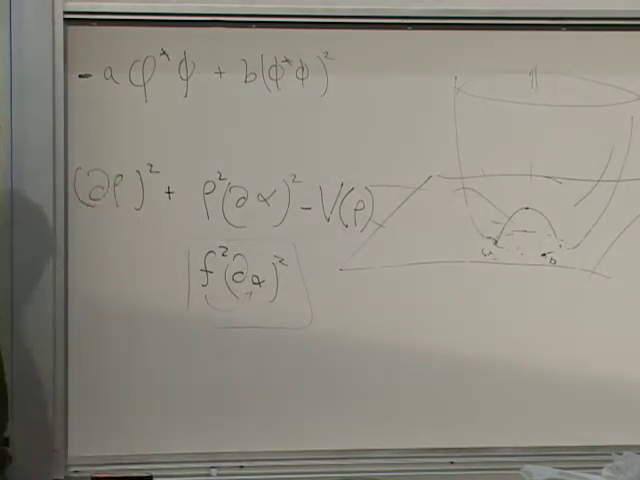
\includegraphics[width=0.88\textwidth]{lecture_07_figure_03.png}
\caption{Die Lagrange-Dichte in Polarkoordinaten, ihr eingerahmter Winkelterm bei niedriger Energie und das Potential mit gebrochener Symmetrie. Radiale Bewegung führt das Potential hinauf; Winkelbewegung folgt der Rinne.}
\lectureframe{00:56:40}
\end{figure}

Bei einer Anregung sehr niedriger Energie bleibt das Feld nahe bei \(\rho=f\). Dann gilt
\begin{equation}
  \mathcal L_{\rm angular}
  \simeq f^2(\partial_\mu\alpha)(\partial^\mu\alpha).
\end{equation}
Bis auf die Konvention für Faktoren von \(1/2\)definieren wir das kanonisch normierte Winkelfeld durch
\begin{equation}
  \beta=\sqrt{2}\,f\alpha,
  \qquad
  \mathcal L_{\rm angular}
  =\frac12(\partial_\mu\beta)(\partial^\mu\beta).
  \label{eq:l07-goldstone-field}
\end{equation}
Es gibt keinen Term \(\beta^2\). Die Quanten dieses Winkelfelds sind masselos. Sie sind die Goldstone-Bosonen.

Das Radialfeld verhält sich anders. Verschiebt man \(\rho\)überall gleichzeitig von \(f\)weg, rollt es zurück, überschwingt die Rinne und oszilliert um sie herum. Für \(\rho=f+h\)ergibt die Entwicklung von Gl.~\eqref{eq:l07-mexican-hat}
\begin{equation}
  V(f+h)=V(f)+\frac12m_h^2h^2+\cdots,
\end{equation}
sodass \(h\)massiv ist. Geometrisch ist die Winkelrichtung flach und die radiale Richtung gekrümmt.

\begin{classroomqa}
\audiencequestion{Wenn das Feld radial ausgelenkt wird, fällt es dann einfach zurück, und was geschieht danach?
\lecturetimestamp{00:57:10}}
\lecturerresponse{Ohne Winkelbewegung fällt es zum Minimum, überschwingt es und oszilliert radial. Eine homogene Oszillation hat verschwindenden räumlichen Impuls, aber eine von null verschiedene Frequenz; diese Frequenz ist die Masse der radialen Anregung. Eine homogene Winkelauslenkung landet dagegen in einem anderen Vakuum und erfährt keine Rückstellkraft.}
\end{classroomqa}

Das ist der Inhalt des Goldstone-Prinzips in diesem Beispiel: Die spontane Brechung einer kontinuierlichen globalen Symmetrie erzeugt für jede unabhängige flache Richtung der Vakuummannigfaltigkeit einen masselosen Modus.
\editorialnote{Die Aussage setzt die üblichen Bedingungen der relativistischen Feldtheorie voraus. In nichtrelativistischen Vielteilchensystemen kann die Zählung und Dispersion von Nambu---Goldstone-Moden subtiler sein, doch die Schlussfolgerung der Vorlesung für große Wellenlängen bleibt für dieses relativistische \(U(1)\)-Modell gültig.}

\section{Spinwellen, Saiten und Schall}

Der Satz ist abstrakt, doch der Mechanismus ist vertraut. In einem isotropen Ferromagneten können alle Spins gemeinsam gedreht werden, ohne die Energie zu ändern. Lässt man die Orientierung über die Probe hinweg sehr langsam variieren, erhält man eine Spinwelle. Ihre Energie geht mit der Wellenzahl gegen null; sie ist daher der Goldstone-Modus der gebrochenen Spin-Rotationssymmetrie.

Eine lange elastische Saite veranschaulicht den Gedanken ebenfalls. Wir vernachlässigen die Schwerkraft und befestigen die Enden so, dass die ganze Saite vertikal verschoben werden kann. Eine gleichförmige vertikale Verschiebung kostet keine Energie. Lässt man die Verschiebung entlang der Saite langsam variieren, entsteht eine Transversalwelle großer Wellenlänge. Die gleichförmige Symmetrieoperation wurde zu einer sanften ortsabhängigen Verformung verallgemeinert.

\begin{figure}[htbp]
\centering
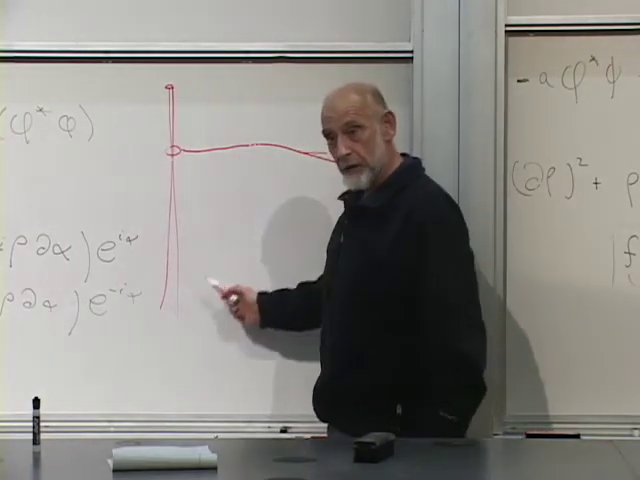
\includegraphics[width=0.68\textwidth]{lecture_07_figure_04.png}
\caption{Das langsam variierende Saitenprofil aus der Analogie zum Goldstone-Modus. Entscheidend ist die geringe Steigung einer Verformung mit großer Wellenlänge, nicht die vertikale Lage der Kurve.}
\lectureframe{01:04:19}
\end{figure}

\begin{classroomqa}
\audiencequestion{Kann die Saite Schwingungsenergie tragen, obwohl sie keinen Impuls hat?
\lecturetimestamp{01:04:41}}
\lecturerresponse{Man muss den vertikalen mechanischen Impuls vom Wellenimpuls entlang der Saite unterscheiden. Eine stehende Welle kann verschwindenden Gesamtimpuls haben, weil sie eine Überlagerung von Moden mit \(+k\)und \(-k\)ist, und dennoch Energie tragen. In der feldtheoretischen Analogie bezieht sich der Impuls auf die Wellenzahl entlang der Achse; die vertikale Auslenkung steht für die innere Feldkoordinate.}
\end{classroomqa}

Eine Slinky-Feder veranschaulicht den longitudinalen Fall. Verschiebt man die gesamte idealisierte unendliche Slinky-Feder entlang ihrer Achse, ändert sich nichts. Verschiebt man benachbarte Teile um geringfügig unterschiedliche Beträge, entsteht eine sanfte Kompressionswelle. In einem Festkörper oder einer Flüssigkeit entsteht langwelliger Schall auf ähnliche Weise durch kollektive Verschiebungen und Dichteänderungen. Spinwellen, transversale Saitenwellen und Schall sind nicht dieselbe mikroskopische Anregung, doch sie weisen dasselbe entscheidende Muster auf: Eine gleichförmige kontinuierliche Operation kostet keine Energie, und ihre langsam variierende Version wird zu einem weichen Modus.
\editorialnote{In einem Kristall werden akustische Phononen üblicherweise als Nambu---Goldstone-Moden der spontan gebrochenen kontinuierlichen Translationssymmetrie beschrieben. Saite und Slinky-Feder dienen in der Vorlesung als mechanische Analogien, die dieselbe Ableitungsstruktur der Energie veranschaulichen.}

Die Bezeichnung verdient einen kurzen Scherz aus der Vorlesung: Es sind \emph{Goldstone}-Bosonen, benannt nach Jeffrey Goldstone, und keine Eichbosonen. Die Vorlesung erwähnt, dass Goldstone ein Freund Susskinds war, und wendet sich dann dem tatsächlich anderen Thema der Eichinvarianz zu.

\section{Von globaler Phasensymmetrie zur Eichsymmetrie}

Die Phasensymmetrie \(U(1)\)ist im Kurs bereits als die mit der Ladungserhaltung verknüpfte Symmetrie aufgetreten. Felder geladener Teilchen sind komplex, und die Multiplikation eines solchen Feldes mit einer gemeinsamen Phase lässt die globale Theorie unverändert. Zur Veranschaulichung kann man von elektrischer Ladung sprechen, doch die Ladung könnte auch eine andere Quantenzahl \(U(1)\)darstellen. Das reale Photon ist masselos; das spätere Ziel ist ein photonartiges Feld wie das massive \(Z\).

Die neue Frage lautet, ob
\begin{equation}
  \phi'(x)=e^{i\theta(x)}\phi(x)
  \label{eq:l07-local-u1}
\end{equation}
eine Symmetrie sein kann, wenn \(\theta\)beliebig durch die Raumzeit variiert. Die Funktion \(\theta(x)\)ist ein Transformationsparameter und kein zusätzliches dynamisches Feld. Wir prüfen den Vorschlag, indem wir ableiten:
\begin{equation}
  \partial_\mu\phi'
  =e^{i\theta}
   \left[\partial_\mu\phi+i(\partial_\mu\theta)\phi\right].
  \label{eq:l07-local-derivative}
\end{equation}
Der zusätzliche Term fehlte bei konstantem \(\theta\). Für das konjugierte Feld gilt
\begin{equation}
  \partial_\mu\phi^{*\prime}
  =e^{-i\theta}
   \left[\partial_\mu\phi^*-i(\partial_\mu\theta)\phi^*\right].
\end{equation}
Ihr Produkt lautet
\begin{align}
  \partial_\mu\phi^{*\prime}\partial^\mu\phi'
  ={}&
  \partial_\mu\phi^*\partial^\mu\phi
  i\left(
      \phi\,\partial_\mu\phi^*
      -\phi^*\partial_\mu\phi
    \right)\partial^\mu\theta
  \nonumber\\
  &+\phi^*\phi\,
    \partial_\mu\theta\,\partial^\mu\theta.
  \label{eq:l07-local-failure}
\end{align}
Das Potential bleibt invariant, weil es nur von \(\phi^*\phi\)abhängt; der gewöhnliche kinetische Term ist es jedoch nicht. Eine globale Symmetrie wird nicht automatisch zu einer lokalen.

\begin{classroomqa}
\audiencequestion{Bedeutet dieses Versagen im Mexican-Hat-Bild, dass es Unebenheiten entlang der kreisförmigen Rinne gibt?
\lecturetimestamp{01:19:37}}
\lecturerresponse{Nein. Das Potential kann in Winkelrichtung vollkommen flach bleiben. Die zusätzlichen Kosten entstehen durch Gradienten, wenn sich die Phase von einem Raumzeitpunkt zum anderen unterscheidet. Es handelt sich nicht um eine Verformung der Rinne; vielmehr registriert der gewöhnliche Ableitungsterm die räumliche Variation.}
\end{classroomqa}

\subsection{Das kompensierende Vektorfeld}

Die Wechselwirkungen des Photons \(W\), des \(Z\)-Bosons und der Gluonen werden durch lokale Eichsymmetrien organisiert, nicht bloß durch starre Transformationen. Damit die lokale Phasenoperation eine Symmetrie ist, erweitern wir die Theorie um ein Vierervektorfeld \(A_\mu\). In der Elektrodynamik ist \(A_0\)das skalare Potential; die drei räumlichen Komponenten bilden das Vektorpotential. Aus ihren Ableitungen entstehen das elektrische und das magnetische Feld.

Wir wählen die in sich konsistente Konvention
\begin{equation}
  \phi'=e^{i\theta}\phi,
  \qquad
  A'_\mu=A_\mu-\partial_\mu\theta,
  \qquad
  D_\mu=\partial_\mu+iA_\mu.
  \label{eq:l07-gauge-convention}
\end{equation}
Beim Überprüfen der Aufhebung ändert sich an der Tafel ein Vorzeichen; Gl. \eqref{eq:l07-gauge-convention}legt alle drei Vorzeichen gemeinsam fest. Die Eichkopplung und die Ladung sind vorübergehend in \(A_\mu\)aufgenommen worden.
\editorialnote{Mit expliziter Ladung \(q\)und Kopplung \(g\)kann man schreiben:
\(D_\mu=\partial_\mu+igqA_\mu\)und
\(A'_\mu=A_\mu-(gq)^{-1}\partial_\mu\theta\). In der Vorlesung werden diese Konstanten weggelassen, damit die Aufhebung sichtbar bleibt.}

Für das konjugierte Feld gilt
\begin{equation}
  D_\mu\phi^*=\partial_\mu\phi^*-iA_\mu\phi^*.
\end{equation}
Nun ist
\begin{align}
  D'_\mu\phi'
  &=
  \left(\partial_\mu+iA'_\mu\right)e^{i\theta}\phi
  \nonumber\\
  &=
  e^{i\theta}
  \left[
    \partial_\mu\phi+i(\partial_\mu\theta)\phi
    +i(A_\mu-\partial_\mu\theta)\phi
  \right]
  \nonumber\\
  &=e^{i\theta}D_\mu\phi.
  \label{eq:l07-covariant-transform}
\end{align}
Die unerwünschte Ableitung von \(\theta\)wird durch die Transformation von \(A_\mu\)aufgehoben. Ebenso gilt
\begin{equation}
  D'_\mu\phi^{*\prime}=e^{-i\theta}D_\mu\phi^*.
\end{equation}
Ihr Produkt ist invariant. Das Adjektiv \emph{kovariant}bedeutet, dass sich die Ableitung auf dieselbe einfache Weise transformiert wie das Feld selbst.

\section{Dynamik des Eichfelds}

Würden wir \(A_\mu\)nur einführen, um eine Ableitung zu korrigieren, hätte das Feld keine eigene Dynamik. Der eichinvariante Feldstärketensor ist
\begin{equation}
  F_{\mu\nu}
  =\partial_\mu A_\nu-\partial_\nu A_\mu.
  \label{eq:l07-field-strength}
\end{equation}
Er ist antisymmetrisch, also gilt \(F_{\mu\mu}=0\). Seine Zeit--Raum-Komponenten enthalten das elektrische Feld, seine Raum--Raum-Komponenten das magnetische Feld. In der vertrauten Vektorschreibweise ist die elektromagnetische Energiedichte proportional zu \(\bm E^2+\bm B^2\), während die Lagrange-Dichte in Lorentz-Signatur proportional zu \(\bm E^2-\bm B^2\)ist; die Vorzeichen hängen von der Metrikkonvention ab.

\begin{classroomqa}
\audiencequestion{Wie lauten Energie und Lagrange-Dichte des elektromagnetischen Feldes?
\lecturetimestamp{01:33:20}}
\lecturerresponse{Die Energie wird aus \(E^2+B^2\)gebildet; in der Lagrange-Dichte steht \(E^2-B^2\). Kovariant schreibt man Letztere als ein übliches Vielfaches von \(F_{\mu\nu}F^{\mu\nu}\). Der antisymmetrische Tensor ist die vierdimensionale Rotation des Vektorpotentials.}
\end{classroomqa}

Die Feldstärke ist selbst eichinvariant:
\begin{align}
  F'_{\mu\nu}
  &=
  \partial_\mu(A_\nu-\partial_\nu\theta)
  -\partial_\nu(A_\mu-\partial_\mu\theta)
  \nonumber\\
  &=
  F_{\mu\nu}
  -\partial_\mu\partial_\nu\theta
  +\partial_\nu\partial_\mu\theta
  =F_{\mu\nu}.
  \label{eq:l07-field-strength-invariant}
\end{align}
Die letzte Gleichheit folgt daraus, dass gewöhnliche gemischte partielle Ableitungen vertauschen. Eine übliche eichinvariante Lagrange-Dichte lautet daher
\begin{equation}
  \boxed{
  \mathcal L
  =(D_\mu\phi)^*D^\mu\phi
  -V(\phi^*\phi)
  -\frac14F_{\mu\nu}F^{\mu\nu}}
  \label{eq:l07-scalar-qed}
\end{equation}
bis auf die Vorzeichen- und Normierungskonventionen der Metrik.

\begin{figure}[htbp]
\centering
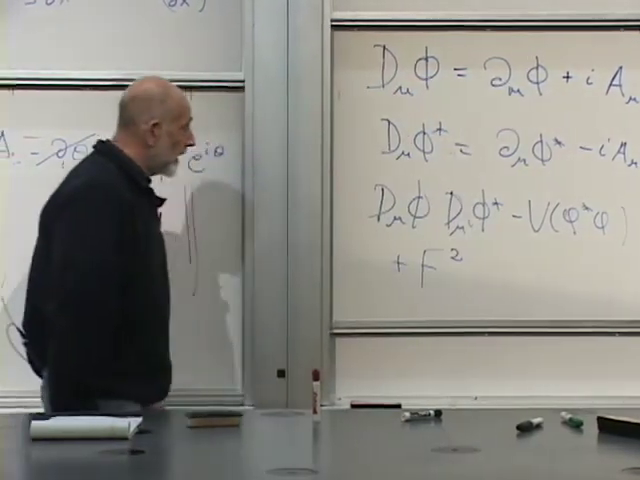
\includegraphics[width=0.84\textwidth]{lecture_07_figure_05.png}
\caption{Die kovarianten Ableitungen und die an der Tafel zusammengestellte eichinvariante Lagrange-Dichte. Numerische Faktoren werden dort weggelassen, damit die Transformationsstruktur sichtbar bleibt.}
\lectureframe{01:38:45}
\end{figure}

Diese Konstruktion macht aus einer globalen \(U(1)\)-Symmetrie eine lokale; dafür müssen wir jedoch---oder, physikalisch gesehen, als Geschenk---ein neues Vektorfeld einführen. Im abelschen Beispiel ist dieses Feld das elektromagnetische Potential.

\begin{classroomqa}
\audiencequestion{In der Lagrange-Dichte, von der wir ausgegangen sind, standen gewöhnliche Ableitungen. Warum dürfen wir sie durch kovariante Ableitungen ersetzen und das Ergebnis als die eigentliche Theorie bezeichnen?
\lecturetimestamp{01:42:55}}
\lecturerresponse{Wir konstruieren eine andere, erweiterte Theorie: geladene Materie zusammen mit einem Eichfeld. Die lokale Eichinvarianz legt ihre Kopplung fest. Die resultierende Quantentheorie ist eine in sich schlüssige mathematische Struktur und stimmt damit überein, wie die Natur das Photon und die schwachen Eichfelder organisiert. Eine relativistische Vektorfeldtheorie einfach auf inkonsistente Weise zu koppeln, kann unphysikalische Polarisationen und Verletzungen der Wahrscheinlichkeitserhaltung zur Folge haben; das Eichprinzip ist also keine kosmetische Umschreibung der alten Theorie eines freien Skalarfelds.}
\end{classroomqa}

\begin{classroomqa}
\audiencequestion{Ist das Hinzufügen des neuen Feldes also die entscheidende Begründung für die Modifikation?\lecturetimestamp{01:44:57}}
\lecturerresponse{Ja. Ohne \(A_\mu\) enthält die Ableitung eines lokal gedrehten Feldes einen nicht kompensierten Term \(\partial_\mu\theta\). Mit \(A_\mu\) und seinem Transformationsgesetz funktioniert die Aufhebung. In der Sprache der Geometrie ist \(A_\mu\) eine Verbindung auf einem Bündel; diese weiterführende Mathematik ist real und nützlich, doch die obige Algebra enthält bereits alles, was wir hier benötigen.}
\end{classroomqa}

\section{Warum eine nackte Eichbosonenmasse verboten ist}

Für ein gewöhnliches bosonisches Feld wird eine Masse durch einen quadratischen Term dargestellt. Es liegt nahe, folgenden Term hinzuzufügen:
\begin{equation}
  \Delta\mathcal L_{\rm Proca}
  =\frac12m^2A_\mu A^\mu.
  \label{eq:l07-proca}
\end{equation}
Unter \(A_\mu\mapsto A_\mu-\partial_\mu\theta\) gilt jedoch
\begin{equation}
  A'_\mu A^{\mu\prime}
  =
  A_\mu A^\mu
  -2A^\mu\partial_\mu\theta
  +\partial_\mu\theta\,\partial^\mu\theta,
\end{equation}
sodass Gleichung ~\eqref{eq:l07-proca} nicht eichinvariant ist. Wir können dieser Eichtheorie nicht von Hand eine Masse hinzufügen und dabei ihre lokale Symmetrie bewahren.

\begin{figure}[htbp]
\centering
\includegraphics[width=0.72\textwidth]{lecture_07_figure_07.png}
\caption{Die vorgeschlagene nackte Vektormasse
\(\tfrac12m^2A_\mu A^\mu\). Ihr Versagen unter
\(A_\mu\mapsto A_\mu-\partial_\mu\theta\) ist das Hindernis, das den Higgs-Mechanismus vorbereitet.}
\lectureframe{01:39:48}
\end{figure}

Hier zeigt sich der scheinbare Widerspruch. Die Eichinvarianz erklärt das masselose Photon und schützt die Theorie vor unphysikalischen Freiheitsgraden, doch \(W\) und \(Z\) sind massiv. Der Ausweg kann keine explizite Vektormasse sein. Er muss aus den bereits in einer eichinvarianten Lagrange-Dichte vorhandenen Feldern hervorgehen.

\begin{classroomqa}
\audiencequestion{Entsteht das Goldstone-Boson durch die Einführung der Eichinvarianz selbst?\lecturetimestamp{01:45:51}}
\lecturerresponse{Nein. Das Goldstone-Boson entstand, als eine kontinuierliche \emph{globale} Symmetrie spontan gebrochen wurde, noch bevor das Vektorpotential eingeführt wurde. Sobald die Symmetrie lokal ist, kann eine ortsabhängige Phase durch \(A_\mu\) kompensiert werden. In der gebrochenen Eichtheorie ist der Winkelmodus kein unabhängiges masseloses Teilchen mehr; er liefert die zusätzliche Polarisation des nun massiven Vektorfeldes. In der nächsten Vorlesung wird diese Aussage hergeleitet und nicht bloß verkündet.}
\end{classroomqa}

\begin{classroomqa}
\audiencequestion{Erklärt irgendetwas davon, warum Flüsse mäandrieren?
\lecturetimestamp{01:47:03}}
\lecturerresponse{Ein direkter Zusammenhang ist hier nicht bekannt. Strömungswirbel und sogar die Formen von Organismen lassen sich durchaus mit Methoden der Symmetrie beschreiben, und es sollte uns nie überraschen, feldtheoretischen Ideen an unerwarteten Stellen zu begegnen; diese Vorlesung behauptet jedoch keine Eichtheorie der Flussmäander.}
\end{classroomqa}

\section{Wo die Vorlesung endet}

Nun haben wir die beiden zu Beginn angekündigten Zutaten. Eine kontinuierliche globale Symmetrie mit einem Kreis von Vakuumzuständen besitzt eine flache Winkelrichtung, und ihre langsame Variation ist ein masseloses Goldstone-Feld. Eine lokale Symmetrie erfordert eine Eichverbindung und kovariante Ableitungen; außerdem verbietet sie die direkte Vektormasse in Gleichung ~\eqref{eq:l07-proca}.

Der nächste Schritt besteht darin, das gebrochene Potential aus Gleichung ~\eqref{eq:l07-mexican-hat} innerhalb der eichinvarianten Theorie aus Gleichung ~\eqref{eq:l07-scalar-qed} zu verwenden. Dann geschehen zwei Dinge zugleich: Das separate Goldstone-Teilchen verschwindet aus dem physikalischen Spektrum, und das Vektorfeld erhält eine Masse. In der üblichen didaktischen Ausdrucksweise wird die Eichsymmetrie spontan gebrochen; genauer gesagt bleibt die Eichredundanz bestehen, während die Theorie in eine Higgs-Phase mit einer massiven Vektoranregung eintritt.
\editorialnote{Eine lokale Eichsymmetrie ist eine Redundanz der Beschreibung und keine gewöhnliche physikalische Symmetrie, die zwischen verschiedenen beobachtbaren Zuständen wirkt. Die Vorlesung verwendet die übliche Kurzform der spontanen Eichsymmetriebrechung. Die eichinvariante physikalische Aussage ist die Neuordnung der Freiheitsgrade in der Higgs-Phase.}

Das ist das Higgs-Phänomen. Wir haben es noch nicht durchgeführt. Diese Vorlesung hat die notwendige, anspruchsvollere Arbeit geleistet: Sie hat das Problem so präzise gefasst, dass die Lösung, wenn sie kommt, unausweichlich sein wird.